\chapter{Sistema de normalización}
\label{ch:Normalizacion}

El circuito realizado para la linealización se basa en el formato IEEE 754, sin embargo el estimador de parámetros que se tiene, esta basado en un formato punto fijo, de manera que se debe considerar una conversión entre ambos formatos, para esto se estudió como pasar de punto flotante a punto fijo, ambos en 32-bits.


\section{Sistema de conversión y normalización }

\begin{figure}[H]
  \centering
    \includegraphics[scale=0.6]{./FF_normalizador.png}
    \rule{35em}{0.5pt}
  \caption[Bloque general del convertidor puto flotante a punto fijo y normalizador]{Bloque general del convertidor puto flotante a punto fijo y normalizador. }
  \label{fig:FF-NORM}
\end{figure}


La figura \ref{fig:FF-NORM} contiene el bloque general del sistema de conversión y normalización , este posee 4 entradas: CLK , F , Begin\_FF , RST\_FF y 2 salidas: ACK\_FF , RESULT.

\begin{figure}[H]
  \centering
    \includegraphics[scale=0.6]{./FMS_FF_NORMALIZADOR.png}
    \rule{35em}{0.5pt}
  \caption[Sistema de convesión, normalización, señales de datos y control]{Sistema de conversión, normalización, señales de datos y control.}
  \label{fig:FMS_FF_NORM}
\end{figure}

El sistema de conversión y normalización de la figura \ref{fig:FMS_FF_NORM} cuenta con dos módulos principales: 

\begin{compactitem}

\item \nt{Convertidor-Normalizador}: En este realizan todas las operaciones requeridas para la conversión del formato Punto flotante- Punto fijo y de la normalización, este se encarga del manejo de los datos en el cálculo. 


\item \nt{Control}: Este se encarga de proveer las señales de control requeridas por el Convertidor-Normalizador, según las condiciones que se tenga y se requiera en cada estado.

\end{compactitem}

señales de datos: 

\begin{compactitem}

\item \nt{F}: Dato de entrada, este posee un valor en formato IEEE 754.
\item \nt{RESULT}: Dato de salida convertido de punto flotante a punto fijo.

\end{compactitem}

señales de control: 

\begin{compactitem}

\item \nt{CLK}: Reloj del sistema, este ejecuta ciclos de reloj con una frecuencia preestablecida. 

\item \nt{Begin\_FF}: Este se encarga de iniciar la la unidad, indica a la maquina de estados que inicia la secuencia. 

\item \nt{RST\_FF}: Este se encarga reestablecer los valores iniciales del sistema de conversión y normalización.

\item \nt{ACK\_FF}: Indica cuando la conversión y la normalización han sido realizadas.

\end{compactitem}


 

\section{Convertidor punto flotante - punto fijo y normalizador }


\begin{figure}[H]
  \centering
    \includegraphics[scale=0.5]{./conversion_FF.png}
    \rule{35em}{0.5pt}
  \caption[conversión y normalización]{Proceso de conversión y normalización  }
  \label{fig:FF}
\end{figure}



  En la figura \ref{fig:FF} se puede observar el diagrama de solución que se utilizó para el desarrollo del convertidor-normalizador , primeramente ingresa el numero en formato IEEE 754 32-bits, posteriormente se efectúa la conversión a punto fijo, en donde se asigna un bit de signo, 5 bits de parte entera y 26 bits para la parte fraccionaria, este dato se procesa en una etapa de normalización y se obtiene el resultado, este valor final esta normalizado para la corriente y tension del panel, $\ V = [0,1]$ e $\ i = [-1,1]$, para el formato punto fijo solo se requiere, un bit de signo, un bit en la parte entera y 30 para la parte fraccionaria, como se muestra en la figura \ref{fig:FF}, el aumento de bits en la parte fraccionaria indica una mejor precisión en el resultado. 

  
  \begin{figure}[H]
  \centering
    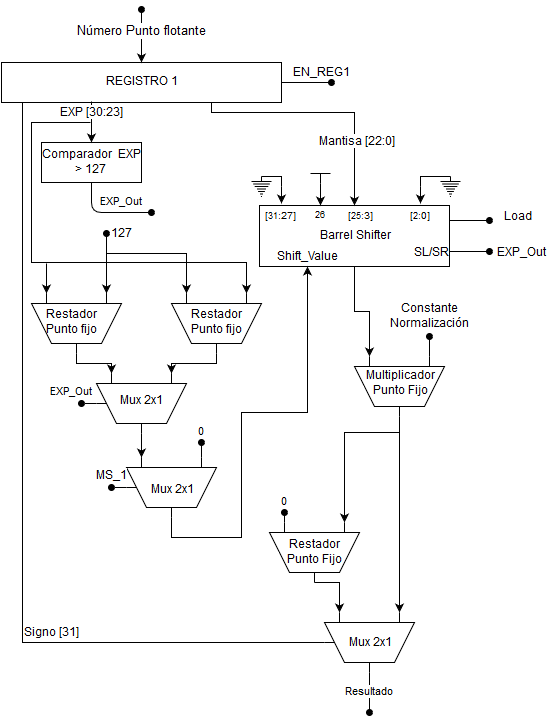
\includegraphics[scale=0.7]{./NORMALIZADOR.png}
    \rule{35em}{0.5pt}
  \caption[Normalizador]{Conversión punto flotante a punto fijo y normalización  }
  \label{fig:NORM}
\end{figure} 

Como se observa en la figura \ref{fig:NORM}, la etapa de conversión de formatos contiene un comparador, este se utiliza para saber si el numero en formato IEEE 754, contiene un exponente mayor o menor que 127, si el numero es igual a 127, indica un exponente de 0, si es mayor la bandera de salida del comparador es igual a 1, $\ EXP\_Out = 1$ , si se da esta condición, se debe realizar la operación $\ EXP - 127$, si el exponente es menor que 127, la bandera $\ EXP\_Out$  es 0 y la operación es $\ 127 - EXP$, ambas operaciones indican la cantidad de desplazamientos que se deben realizar en el Barrel-shifter, este se utiliza debido a que es puramente combinacional, por lo que no requiere ciclos de reloj para funcionar, esto disminuye el tiempo de calculo en la etapa de conversión, la direccion de los desplazamientos se puede controlar mediante una señal de control que posee, esta es conectada a la bandera del comparador  $\ EXP\_Out $, el dato de entrada para el barrel-shifter esta compuesto por un bit mas significativo fijo en alto y los 23 bits de la mantisa del dato de entrada en punto flotante, este dato compuesto del barrel-shifter se le aplican los desplazamientos para obtener el resultado en punto fijo, este resultado siempre es positivo, debido a que en esta etapa no se contempla el signo, se retomara en otra etapa.    

Un dato normalizado requiere una division entre el maximo valor que se puede procesar, sin embargo en un circuito digital las divisiones se tornar complicadas y requieren de mucha area, por lo que utiliza una multiplicación por una constante, esta etapa de normalización  posee un multiplicador en punto fijo, las entradas de este contienen el valor convertido en punto fijo y una constante de normalización, esta constante se calcula en la siguiente ecuación: 
      

\begin{equation} \label{eq:ej1}
  C_{norm}
  = \frac{1}{Valor_{MAX}}  
\end{equation}  

La etapa de conversión y normalización se utiliza tanto para la corriente $\ i_{pv} $ como para la tensión $\ V_{pv} $ del panel, esta constante de normalización varia para cada circuito:
  
\begin{equation} \label{eq:ej2}
  Cv_{norm}
  = \frac{1}{18.1} = 0.055248618  
\end{equation}

\begin{equation} \label{eq:ej3}
  Ci_{norm}
  = \frac{1}{Ln\left(0.00667769\right)} = 0.199641045  
\end{equation}
 
 Donde $\ Cv_{norm}$ es la constante de normalización de la tensión y $\ Ci_{norm}$ la constante de normalización de la corriente. 
 
 Posteriormente a la normalización, se debe tomar en cuenta el signo del valor inicial punto flotante, el formato IEEE 754 contiene el signo en el bit mas significativo (bit 32), en la unidad de conversion-normalización se realiza la resta $0-Dato\_Punto\_fijo$, y el multiplexor 2x1 del resultado selecciona el valor final en punto fijo, si el bit 32 del valor inicial punto flotante es cero, el valor final en punto fijo es positivo, de lo contrario el valor final en punto fijo es negativo. 
  
\section{Control}

La arquitectura diseñada para el convertidor-normalizador en su mayoría es combinacional sin embargo requiere un control, que detecta si se deben realizar  desplazamientos, y cuando se debe almacenar datos en registros. 

\begin{figure}[H]
  \centering
    \includegraphics[scale=0.6]{./MaquinaFF.png}
    \rule{35em}{0.5pt}
  \caption[Maquina de estados finita para el convetidor-normalizador]{Maquina de estados finita para el convertidor-normalizador}
  \label{fig:CTRLNORM}
\end{figure} 

El control de esta arquitectura se realiza por medio de una máquina de estado finita bastante sencilla, donde básicamente se cuenta con cuatro acciones principales, el primer estado (a) espera que la unidad sea  iniciada mediante la señal $\ Begin\_FF$ y se ejecuta un reset en los registros, el estado (b) guarda el dato en el \nt{Registro 1}, el estado (c) verifica la condición $\ EXP=127 $ con esta se determina si se deben realizar desplazamientos, el estado (f) almacena en el Barrel-shifter el dato convertido, el estado (g) almacena el resultado final en el \nt{Registro 2} y en el estado (h) se indica mediante la bandera $\ ACK\_FF$ que el dato ya fue convertido y normalizado.

\section{Sistema de conversión-normalización en verilog}

Este circuito se implementó por medio de el lenguaje de descripción de hardware "Verilog", inicialmente se realizaron pequeños bloques pertenecientes a cada elemento requerido por la arquitectura diseñada, se implementa la unidad de conversión-normalización y la unidad de control en bloques separados, de manera que se pudieran realizar pruebas sin dependencia de los bloques entre si, para una mejor depuración de errores y re-diseño, finalmente se realizan las simulaciones al bloque completo en la figura \ref{fig:SIMNORM}. 

\begin{figure}[H]
  \centering
    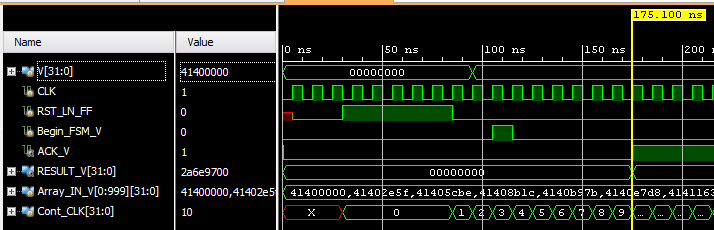
\includegraphics[scale=0.8]{./TEST_CONV_NOM_I.png}
    \rule{35em}{0.5pt}
  \caption[Simulación del circuito de conversión y normalización]{Simulación del circuito de conversión y normalización}
  \label{fig:SIMNORM}
\end{figure}

\section{Simulación y verificación del convertidor-normalizador}

En la implementación de un diseño en hardware, es de suma importancia simular y verificar que este funcione de manera adecuada al comportamiento esperado teóricamente. Para la comprobación de la unidad de conversión-normalización, se realizaron una serie de pruebas en donde se programó una simulación ("testbench") que contiene una prueba con mil valores de entrada, ingresados por medio de un archivo de texto previamente editado con los datos de entrada del comportamiento segun el modelo del panel, las pruebas de esta unidad se realizaron con valores de corriente $ i_{pv}$ y valores de tension $ V_{pv}$. 


  \begin{figure}[H]
  \centering
    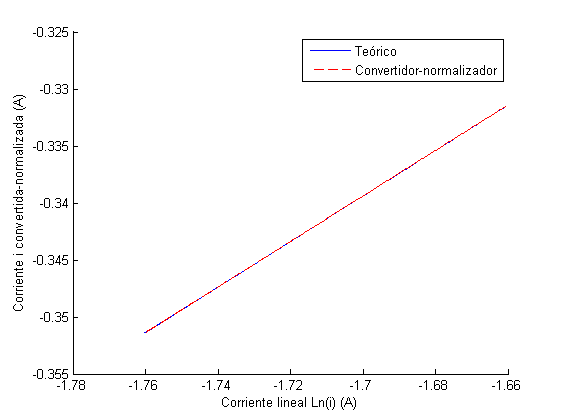
\includegraphics[scale=0.7]{./Convertidor-normalizador_I.png}
    \rule{35em}{0.5pt}
  \caption[Comparación entre la conversión-normalización de corriente $\ i_{pv}$ teórica y del circuito]{Comparación entre la conversión-normalización de corriente $\ i_{pv}$ teórica y del circuito}
  \label{fig:NORMI}
\end{figure}

En la figura \ref{fig:NORMI} se presenta la comparación entre los resultados obtenidos teóricamente y experimentalmente, tomando como datos de entrada  valores de corriente en formato punto flotante y retornando en la salida valores de corriente normalizados y en formato punto fijo. Estos resultados se pueden comparar por medio del porcentaje de error.  

  \begin{figure}[H]
  \centering
    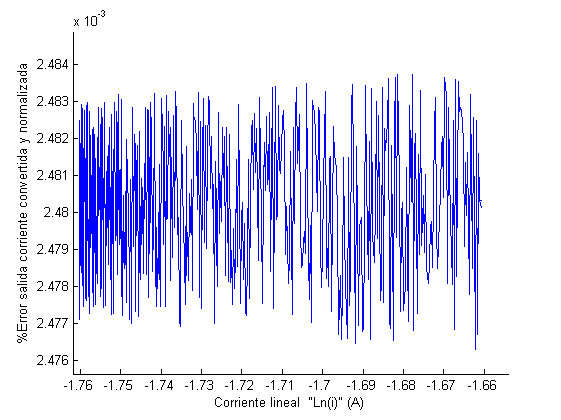
\includegraphics[scale=0.7]{./ERROR_CONV_NORM_I.png}
    \rule{35em}{0.5pt}
  \caption[\%Error entre la conversión-normalización de corriente $\ i_{pv}$ teórica y del circuito]{\%Error entre la conversión-normalización de corriente $\ i_{pv}$ teórica y del circuito}
  \label{fig:ENORMI}
\end{figure}

En la figura \ref{fig:ENORMI} se puede observar el error entre la conversión de la corriente normalizada teórica y experimental, con un error porcentual máximo de 0,0024837\% y un error promedio de 0,002478\% 


  \begin{figure}[H]
  \centering
    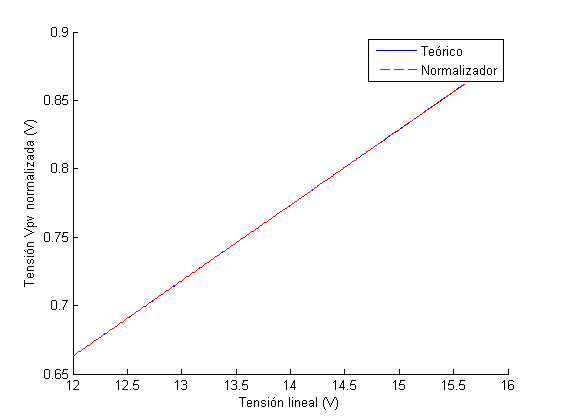
\includegraphics[scale=0.7]{./Normalizador_V.png}
    \rule{35em}{0.5pt}
  \caption[Comparación entre la conversión-normalización de tensión $\ V_{pv}$ teórica y del circuito]{Comparación entre la conversión-normalización de tensión  $\ V_{pv}$ teórica y del circuito}
  \label{fig:NORMV}
\end{figure}


  \begin{figure}[H]
  \centering
    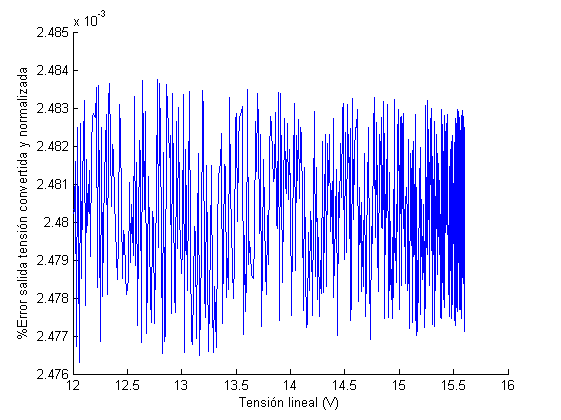
\includegraphics[scale=0.7]{./ERROR_CONV_NORM_V.png}
    \rule{35em}{0.5pt}
  \caption[\%Error entre la conversión-normalización de tensión $\ V_{pv}$ teórica y del circuito]{\%Error entre la conversión-normalización de tensión $\ V_{pv}$ teórica y del circuito}
  \label{fig:ENORMV}
\end{figure}

El análisis utilizado para la conversión-normalización de la corriente se utiliza para los resultados de la tensión, en la figura \ref{fig:NORMV} se muestran los resultados obtenidos con una tension de entrada y su normalizacion tanto teorico como experimental, de la misma manera se puede hacer el calculo del error entre ambas, en la figura \ref{fig:ENORMV} se puede observar el error máximo de 0,0024837\% y un error promedio de 0,002478\%.

Esta unidad contiene muchos bloques combinacionales, por lo que se requieren pocos ciclos de reloj en la maquina de estados para realizar la conversión y la normalización, la maquina de estados finita indica que  se requieren 8 ciclos de reloj para que el resultado sea concluido, con las simulaciones efectuadas al circuito se comprueba como se mostró en la  figura \ref{fig:SIMNORM} 
